\section{Introduction}
\label{sec:introduction}

Globally, it is estimated that people spend approximately 90\% of their time indoors \cite{schweizer_indoor_2007, klepeis_national_2001} and breath 11.000 liters of air per day \cite{corlan_importance_2021}. Suboptimal indoor air quality (IAQ) conditions affect building occupants' experiences of comfort and insufficient ventilation in indoor spaces is proven to play significant roles in occupants' well-being, health and cognitive functions \cite{, wang_how_2021, kim_analyzing_2019}. 

The research into the influence of Indoor Environmental Quality (IEQ) \cite{kulshreshtha_indoor_2024} on occupants', including acoustic, thermal and visual conditions, is gaining more attention espicially the field of indoor ventilation. One core aspect of air quality is its invisibility to occupants \cite{son_perceived_2023}, polluted air is not easily detected by smell or sight. Additionally, mechanical ventilation systems in buildings operate discreetly, contributing to occupants' perceived lack of control since these systems are typically automated and cannot be directly regulated or controlled by occupants themselves. This creates an interplay between occupants' effects onhealth and comfort, architecture and built environments, and computing technologies (see Figure \ref{fig:complexity}).

This thesis focuses on understanding occupants' needs through in-the-wild studies measuring indoor air quality in specific spaces (e.g. meeting rooms) and arprototyping various persuasive technologies and data physicalization devices to visualize indoor air quality and evaluating their effectiveness with the overall goal of gathering insights into occupants' comfort levels and helping them to take preventive action against poor indoor air quality. 

Researching occupants' subjective needs, experiences, and behavior, coupled with a human-centric design approach, has the potential to improve occupants' well-being and create indoor environments with good indoor air quality. Furthermore, it provides valuable insights to faculty staff in making decisions in setting up ventilation systems, arranging indoor spaces, and informing architecture and interior design studios on making decisions about structuring spaces and integrating computing technologies within built environments.

While research on defining comfort within indoor buildings, gathering and analyzing sensory indoor climate data, and the effects of poor air quality are prevalent, there is a gap in understanding occupants' behavior and their subjective needs, along with limited research on how design solutions visualize environmental data and computing installations can empower occupants, particularly within the field of physically visualizing data to convey IAQ to building occupants in real-time.

\begin{figure}[h]
    \centering
    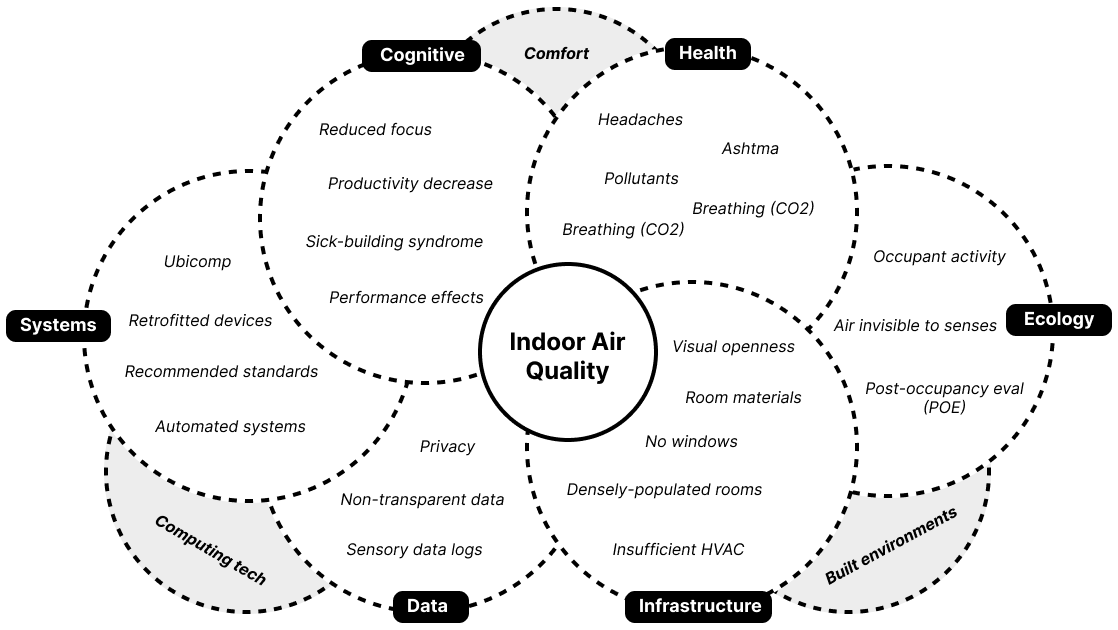
\includegraphics[width=0.5\textwidth]{complexity_diagram_indoor_air_quality.png}
    \caption{Complexity diagram providing an overview of the effects of IAQ and needs of occupants \cite{schweizer_indoor_2007, wang_how_2021, kim_analyzing_2019}}
    \label{fig:complexity}
\end{figure}



\subsection{Research questions}

In order to research intervention strategies for improving indoor air quality, the following main research question is formulated: \\

\emph{\textbf{RQ:} How can real-time sensory measurements and future predictions of air quality be physically visualised in specific indoor spaces integrating both environmental information and elements that increase awareness among occupants facilitating their adoption of preventive measures against poor air quality?} \\

To effectively answer this main research question, this research is guided by the following supporting sub-questions that also serve as objectives to delineate the necessary knowledge: \\

\begin{itemize}
    \item \textbf{SRQ1:} \emph{How can environmental information related to air quality, such as pollutant concentrations and ventilation rates, be incorporated into the visual representations?}
    \item \textbf{SRQ2:} \emph{How do different types of physical visualizations impact occupants' understanding of air quality and their willingness to adopt preventive measures?}
    \item \textbf{SRQ3:} \emph{How do occupants' perceptions and behaviors regarding indoor air quality change over time, from pre to post-installation of the physical representation of poor air quality?}\\
\end{itemize}